\batchmode
\makeatletter
\def\input@path{{"C:/Users/tkpme/Dropbox/BookPCRA/Springer Production March 2026/Ch Appendix D Portfolio Theory/"}}
\makeatother
\documentclass[graybox,envcountchap,sectrefs]{svmono}\usepackage[]{graphicx}\usepackage[]{xcolor}
% maxwidth is the original width if it is less than linewidth
% otherwise use linewidth (to make sure the graphics do not exceed the margin)
\makeatletter
\def\maxwidth{ %
  \ifdim\Gin@nat@width>\linewidth
    \linewidth
  \else
    \Gin@nat@width
  \fi
}
\makeatother

\definecolor{fgcolor}{rgb}{0.345, 0.345, 0.345}
\newcommand{\hlnum}[1]{\textcolor[rgb]{0.686,0.059,0.569}{#1}}%
\newcommand{\hlsng}[1]{\textcolor[rgb]{0.192,0.494,0.8}{#1}}%
\newcommand{\hlcom}[1]{\textcolor[rgb]{0.678,0.584,0.686}{\textit{#1}}}%
\newcommand{\hlopt}[1]{\textcolor[rgb]{0,0,0}{#1}}%
\newcommand{\hldef}[1]{\textcolor[rgb]{0.345,0.345,0.345}{#1}}%
\newcommand{\hlkwa}[1]{\textcolor[rgb]{0.161,0.373,0.58}{\textbf{#1}}}%
\newcommand{\hlkwb}[1]{\textcolor[rgb]{0.69,0.353,0.396}{#1}}%
\newcommand{\hlkwc}[1]{\textcolor[rgb]{0.333,0.667,0.333}{#1}}%
\newcommand{\hlkwd}[1]{\textcolor[rgb]{0.737,0.353,0.396}{\textbf{#1}}}%
\let\hlipl\hlkwb

\usepackage{framed}
\makeatletter
\newenvironment{kframe}{%
 \def\at@end@of@kframe{}%
 \ifinner\ifhmode%
  \def\at@end@of@kframe{\end{minipage}}%
  \begin{minipage}{\columnwidth}%
 \fi\fi%
 \def\FrameCommand##1{\hskip\@totalleftmargin \hskip-\fboxsep
 \colorbox{shadecolor}{##1}\hskip-\fboxsep
     % There is no \\@totalrightmargin, so:
     \hskip-\linewidth \hskip-\@totalleftmargin \hskip\columnwidth}%
 \MakeFramed {\advance\hsize-\width
   \@totalleftmargin\z@ \linewidth\hsize
   \@setminipage}}%
 {\par\unskip\endMakeFramed%
 \at@end@of@kframe}
\makeatother

\definecolor{shadecolor}{rgb}{.97, .97, .97}
\definecolor{messagecolor}{rgb}{0, 0, 0}
\definecolor{warningcolor}{rgb}{1, 0, 1}
\definecolor{errorcolor}{rgb}{1, 0, 0}
\newenvironment{knitrout}{}{} % an empty environment to be redefined in TeX

\usepackage{alltt}
\usepackage{mathptmx}
\usepackage{helvet}
\usepackage{courier}
\usepackage[T1]{fontenc}
\usepackage[utf8]{inputenc}
\usepackage{geometry}
\geometry{verbose,tmargin=1in,bmargin=1in,lmargin=1in,rmargin=1in}
\setcounter{tocdepth}{3}
\setlength{\parskip}{\medskipamount}
\setlength{\parindent}{0pt}
\usepackage{float}
\usepackage{textcomp}
\usepackage{amsmath}
\usepackage{amssymb}
\usepackage{graphicx}
\usepackage[unicode=true,pdfusetitle,
 bookmarks=true,bookmarksnumbered=true,bookmarksopen=true,bookmarksopenlevel=1,
 breaklinks=false,pdfborder={0 0 1},backref=false,colorlinks=false]
 {hyperref}
\hypersetup{
 pdfstartview=XYZ null null 1.25,pdfpagemode=UseNone}

\makeatletter
%%%%%%%%%%%%%%%%%%%%%%%%%%%%%% User specified LaTeX commands.
%%%%%%%%%%%%%%%%%%%% book.tex %%%%%%%%%%%%%%%%%%%%%%%%%%%%%
%
% sample root file for the chapters of your "monograph"
%
% Use this file as a template for your own input.
%
%%%%%%%%%%%%%%%% Springer-Verlag %%%%%%%%%%%%%%%%%%%%%%%%%%


% RECOMMENDED %%%%%%%%%%%%%%%%%%%%%%%%%%%%%%%%%%%%%%%%%%%%%%%%%%%


% choose options for [] as required from the list
% in the Reference Guide

\usepackage{makeidx}% allows index generation
% standard LaTeX graphics tool
                             % when including figure files
\usepackage{multicol}% used for the two-column index
\usepackage[bottom]{footmisc}% places footnotes at page bottom

\usepackage{hyperref}
\def\UrlBreaks{\do\/\do-}

% see the list of further useful packages
% in the Reference Guide

\makeindex             % used for the subject index
                       % please use the style svind.ist with
                       % your makeindex program


%\usepackage[ style=authoryear,natbib=true,giveninits=true,backend=biber,maxcitenames=2]{biblatex}
\usepackage[style=authoryear,natbib=true,firstinits=false,backend=biber,maxcitenames=2]{biblatex}


\setlength{\bibitemsep}{0.5\baselineskip}
\DeclareNameAlias{sortname}{family-given}

\IfFileExists{C:/Users/Doug/Dropbox/BookPCRA/mpslbookCombined.bib}
{\addbibresource[location=local]{C:/Users/Doug/Dropbox/BookPCRA/mpslbookCombined.bib}}
{   \IfFileExists{C:/Users/tkpme/Dropbox/BookPCRA/mpslbookCombined.bib}
    {\addbibresource[location=local]{C:/Users/tkpme/Dropbox/BookPCRA/mpslbookCombined.bib}}
    {   \IfFileExists{C:/Users/stoya/Dropbox/BookPCRA/mpslbookCombined.bib}
        {\addbibresource[location=local]{C:/Users/stoya/Dropbox/BookPCRA/mpslbookCombined.bib}}
        {   \IfFileExists{C:/Users/4thauthor/Dropbox/BookPCRA/mpslbookCombined.bib}
            {\addbibresource[location=local]{C:/Users/4thauthor/Dropbox/BookPCRA/mpslbookCombined.bib}}
            {}
        }
    }
}
\renewcommand\cite{\citet}

\usepackage{amsmath}
\usepackage{amssymb}
\usepackage[p,osf]{stickstootext}
\usepackage[stix2,vvarbb]{newtxmath}
\usepackage[varqu,varl]{inconsolata}
% \usepackage{txfonts}
\usepackage{upgreek}

\DeclareMathOperator{\argmax}{arg\,max}
\DeclareMathOperator{\argmin}{arg\,min}
\usepackage{array}
\usepackage{arydshln}
\usepackage{booktabs}
\usepackage{threeparttablex}
\usepackage{appendix}

\usepackage[utf8]{inputenc}
%%%%%%%%%%%%%%%%%%%%%%%%%%%%%%%%%%%%%%%%%%%
\IfFileExists{C:/Users/Doug/Dropbox/BookPCRA/macroSP_August_05_2021.tex}
{\input{C:/Users/Doug/Dropbox/BookPCRA/macroSP_August_05_2021.tex}}
{   \IfFileExists{C:/Users/tkpme/Dropbox/BookPCRA/macroSP_August_05_2021.tex}
    {\input{C:/Users/tkpme/Dropbox/BookPCRA/macroSP_August_05_2021.tex}}
    {   \IfFileExists{C:/Users/stoya/Dropbox/BookPCRA/macroSP_August_05_2021.tex}
        {\input{C:/Users/stoya/Dropbox/BookPCRA/macroSP_August_05_2021.tex}}
        {   \IfFileExists{C:/Users/4thAuthor/Dropbox/BookPCRA/macroSP_August_05_2021.tex}
            {\input{C:/Users/4thAuthor/Dropbox/BookPCRA/macroSP_August_05_2021.tex}}
            {}
        }
    }
}

\belowsink=90pt


%%%%%%%%%%%%%%%%%%%%%%%%%%%%%%%%%%%%%%%%%%%%%

\makeatother
\IfFileExists{upquote.sty}{\usepackage{upquote}}{}
\begin{document}
\begin{appendices}


\setcounter{chapter}{3} 

\chapter{PORTFOLIO THEORY\label{chap:AppendixD}}

\vspace{0.3in}

\textbf{Planned for publication in 2026 by R. Douglas Martin, Thomas
K. Philips, Bernd Scherer and Kirk Li. All rights reserved. © Copyright
2025}

\vspace{0.3in}

\begin{center}
10/12/25
\par\end{center}

\tocchpnum=30pt 
\tocsecnum=33pt 
\tocsubsecnum=40pt 
\tocsubsubsecnum=48pt 
\tocparanum=55pt 
\tocsubparanum=63pt
\calctocindent

\tableofcontents{}\newpage{}

\section{MinVar Frontier Mathematics\label{sec: minVarMath}}

In \GlobalMinVarPortfolios\ we showed that the weight vector $\mathbf{w}_{mv}$
that minimize portfolio variance, subject to the mean return and full
investment constraints $\mathbf{w}^{\prime}\bumu=\mu_{P}$ and $\mathbf{w}^{\prime}\mathbf{1}=1$,
has the form

\begin{equation}
\mathbf{w}_{\mathrm{mv}}=\lambda_{1}\mathbf{C}^{-1}\bumu\,+\,\lambda_{2}\mathbf{C}^{-1}\boldsymbol{1}.\label{eq: minVarWtVectorGeneralForm}
\end{equation}

Applying the mean return and full-investment constrains results in
two equations in the two unknowns $\lambda_{1}$ and $\lambda_{2}$,
and the reader can easily show that the solution to these equations
is

\begin{equation}
\begin{alignedat}{1}\lambda_{1} & =\dfrac{c\mu_{P}\,-\,a}{d}\\
\lambda_{2} & =\dfrac{b\,-\,a\mu_{P}}{d}
\end{alignedat}
\label{eq: theTwoLamdas}
\end{equation}

where $a=\mathbf{1}^{\prime}\mathbf{C}^{-1}\bumu$, $b=\bumu^{\prime}\mathbf{C}^{-1}\bumu$,
$c=\mathbf{1}^{\prime}\mathbf{C}^{-1}\mathbf{1}>0$, and $d=bc\,-\,a^{2}$.

Substituting $\lambda_{1}$ and $\lambda_{2}$ into \eqref{eq: minVarWtVectorGeneralForm}
and easy algebraic manipulation results in

\begin{equation}
\mathbf{w}_{\mathrm{mv}}=\mathbf{w}_{1}\,+\,\mu_{P}\mathbf{w}_{2}\label{eq: minVarWtVector}
\end{equation}

where

\begin{equation}
\begin{alignedat}{1}\mathbf{w}_{1} & =\dfrac{1}{d}\left(b\mathbf{C}^{-1}\mathbf{1}\,-\,a\mathbf{C}^{-1}\bumu\right)\\
\mathbf{w}_{2} & =\dfrac{1}{d}\left(c\mathbf{C}^{-1}\bumu\,-\,a\mathbf{C}^{-1}\mathbf{1}\right).
\end{alignedat}
\label{eq: minVarPairOfWts}
\end{equation}

and

\begin{align}
d & =(\bumu^{\mathrm{\prime}}\mathbf{C}^{-1}\bumu)({\bf 1^{\mathrm{\prime}}}\mathbf{C}^{-1}{\bf 1})\,-\,{\bf ({\bf 1^{\mathrm{\prime}}}}\mathbf{C}^{-1}\bumu)^{2}\label{eq: dExpression}\\
 & \geqslant0
\end{align}

where we show below how the above inequality follows from the Cauchy-Schwarz
inequality, and that $d$ is positive except in the special case where
$\bum=c\mathbf{1}$ for some constant $c$, which does not arise in
practice. 

Also, we note that

\begin{equation}
\begin{alignedat}{1}c^{-1} & =\sigma_{\mathrm{gmv}}^{2}\\
\dfrac{a}{c} & =\mu_{\mathrm{gmv}}
\end{alignedat}
\label{eq: constantsMore}
\end{equation}

where $\mu_{\mathrm{gmv}}$ and $\sigma_{\mathrm{gmv}}^{2}$ are the
mean and variance of the global minimum variance (GMV) portfolio.

\subsubsection*{Positivity of $\boldsymbol{d}$\label{subsec: positivity of d}}

Since $\mathbf{C}$ is positive definite so is $\mathbf{C}^{-1}$,
and basic matrix theory shows that therefore $\mathbf{C}^{-1}$ can
be factored into the product of two inverse square root matrices,
$\mathbf{C}^{-1}=\mathbf{C}^{-1/2}\mathbf{C}^{-1/2}$ where $\mathbf{C}^{-1/2}$
is positive definite. Thus one has

\begin{align*}
d & =(\bumu^{\mathrm{\prime}}\mathbf{C}^{-1/2}\mathbf{C}^{-1/2}\bumu)\,\cdot\,({\bf 1^{\mathrm{\prime}}}\mathbf{C}^{-1/2}\mathbf{C}^{-1/2}{\bf 1})\,-\,{\bf ({\bf 1^{\mathrm{\prime}}}}\mathbf{C}^{-1/2}\mathbf{C}^{-1/2}{\bf \boldsymbol{\mu}})^{2}\\
 & =(\check{\bumu^{\prime}}\check{\bumu})\,\cdot\,(\check{\mathbf{1}}^{\mathrm{\prime}}\check{\mathbf{1}})\,-\,(\check{\mathbf{1}}^{\mathrm{\prime}}\check{{\bf \bumu}})^{2}
\end{align*}

where $\check{\bumu}=\mathbf{C}^{-1/2}\bumu$ and $\check{\mathbf{1}}=\mathbf{C}^{-1/2}{\bf 1}$.
The Cauchy-Schwarz inequality for two vectors $\mathbf{x}$ and $\mathbf{y}$
states that

\begin{equation}
{\bf ({\bf x^{\mathrm{\prime}}}}\mathbf{y})^{2}\leqslant{\bf ({\bf x^{\mathrm{\prime}}}}\mathbf{x})\,\cdot\,{\bf ({\bf y^{\mathrm{\prime}}}}\mathbf{y})\quad\mathrm{with\:equality\:if,\:and\:only\:if,}\quad\mathbf{y=\mathrm{\mathit{c\cdot\mathbf{x}}}}
\end{equation}

for some non-zero constant $c$. Thus $d$ is equal to zero if and,
only if, $\mathbf{C}^{-1/2}\bumu=c\cdot\mathbf{C}^{-1/2}{\bf 1}$,
equivalently if and only if $\mathbf{C}^{-1/2}\left(\bumu\,-\,c\cdot\mathbf{1}\right)={\bf 0}$,
where $\mathbf{0}$ is a vector of zeros. But since $\mathbf{C}^{-1/2}$
is positive definite, the condition $\mathbf{C}^{-1/2}\left(\bumu\,-\,c\cdot\mathbf{1}\right)={\bf 0}$
can only occur if $\bumu=c\,\cdot\,\mathbf{1}$. Thus $d=0$ if, and
only if, the portfolio mean vector has all equal values, which essentially
never happens in practice.

\section{The Tangent Portfolio is the Market Portfolio Under the CAPM\label{sec: tangentPortIsMktPortUnderCAPM}}

Under the first CAPM assumption in \CAPM, all market participants
hold the tangent portfolio $T$, and the last assumption implies that
the supply of securities equals the demand. Let $N$ be the number
of securities in the market, with $V_{j}$ be the market capitalization
of the $j^{th}$ security. Then $V=\sum_{j\,=\,1}^{N}V_{j}$ is the
total market capitalization, and $w_{M,\,j}=V_{j}/V$ is the weight
of the $j^{th}$ security in the market portfolio. Let $K$ be the
number of market investors, where the $k^{th}$ investor invests an
amount $\gamma_{k}W_{k},\ 0<\gamma_{k}<1$ in risky assets and an
amount $W_{k}(1-\gamma_{k})$ in the risk-free asset. In general the
$k^{th}$ investor would invest an amount $\gamma_{k}W_{k}w_{k,\,j}$
in the $j^{th}$ market asset, and therefore the total amount invested
in the $j^{th}$ asset by all investors is

\[
\dot{V}_{j}=\sum_{k\,=\,1}^{K}\gamma_{k}\,W_{k}\,w_{k,\,j}.
\]

However, under the CAPM assumptions all investors all hold the same
tangent portfolio, so $w_{k,\,j}=w_{j},\,k=1,\,2\,,\cdots,\,K$ where
$w_{j}$ is the weight of the $j^{th}$ asset in the tangent portfolio
$T$, and $\sum_{j\,=\,1}^{N}w_{j}=1$. Thus

\[
\dot{V}_{j}=w_{j}\sum_{k\,=\,1}^{K}\gamma_{k}\,W_{k}
\]

is the amount invested by all investors in the $j^{th}$ asset, and
$\dot{V}=\sum_{j\,=\,1}^{N}\dot{V}_{j}=\sum_{k\,=\,1}^{K}\gamma_{k}\,W_{k}$
is the total amount invested by all investors. However, under the
CAPM equilibrium assumption $\dot{V}_{j}=V_{j}$ and $\dot{V}=V$,
which results in

\[
w_{M,\,j}=\dfrac{V_{j}}{V}=\dfrac{\dot{V}_{j}}{\dot{V}}=w_{j},\ j=1,\,2,\,\cdots\,,\,N
\]

and so the tangent portfolio $T$ is the market portfolio $M$.

\section{Proof of the CAPM\label{subsec: CAPMproof}}

The following is a simple proof of the CAPM formula \CAPMformula
with beta defined by \CAPMbeta. Let $M$ be the market portfolio
whose mean return and variance are $\mu_{M}$ and $\sigma_{M}^{2}$
respectively. As the market portfolio is the tangent portfolio, the
Capital Allocation Line associated with the entire market is known
as the \emph{Capital Market Line} (CML), and can be written as 

\begin{equation}
\mu=r_{f}\,+\,\dfrac{(\mu_{M}\,-\,r_{f})}{\sigma_{M}}\sigma.\label{eq: CML}
\end{equation}

Now consider any security in the market place with return $r_{i}$,
mean $\mu_{i}$ and variance $\sigma_{i}^{2}$, such that $(\mu_{i},\sigma_{i})$
does not lie on the efficient frontier. We form a portfolio $P$ by
investing a fraction $\alpha$ in the security and a fraction $1-\alpha$,
in the market portfolio $M$. The mean return and variance of the
portfolio $P$ are:

\begin{align*}
\mu_{P} & =\alpha\mu_{i}\,+\,(1\,-\,\alpha)\mu_{M}\\
\sigma_{P} & =\left(\alpha^{2}\sigma_{i}^{2}\,+\,2\,\alpha\,(1\,-\,\alpha)\,\sigma_{i,\,M}\,+\,(1\,-\,\alpha)^{2}\sigma_{M}^{2}\right)^{1/2}.
\end{align*}

The pair $(\mu_{P},\,\sigma_{P})=(\mu_{P}(\alpha),\,\sigma_{P}(\alpha))$
traces out a $\mu_{P}(\alpha)$ versus $\sigma_{P}(\alpha)$ curve
in portfolio mean return versus standard deviation space as $\alpha$
varies from $0$ to $1$, with value $(\mu_{i},\,\sigma_{i})$ when
$\alpha=1$ and value $(\mu_{M},\,\sigma_{M})$ when $\alpha=0$.
This curve can never lie above or to the left of the CML (if it did,
the CML would not be optimal), and the slope of the curve at $\alpha=0$
is

\begin{align}
\dfrac{d\mu}{d\sigma}(\alpha)\Biggr|_{\alpha=0} & =\dfrac{d\mu/d\alpha\bigr|_{\alpha=0}}{d\sigma/d\alpha\bigr|_{\alpha=0}},\label{eq: DmuDsigmaFunction}
\end{align}

where the derivative of the numerator is equal to $\mu_{i}\,-\,\mu_{M}$
for all $\alpha$ including $\alpha=0$. Straightforward calculus
yields an expression for $d\sigma/d\alpha$ that reduces to $\left(\sigma_{i,\,M}\,-\,\sigma_{M}^{2}\right)/\sigma_{M}$
when $\alpha=0$. Thus

\begin{equation}
\dfrac{d\mu}{d\sigma}(\alpha)\Biggr|_{\alpha=0}=\sigma_{M}\dfrac{\mu_{i}\,-\,\mu_{M}}{\sigma_{i,\,M}\,-\,\sigma_{M}^{2}}\label{eq: DmuDsigmaAtMarketPort}
\end{equation}

A small but important step in the proof is a straightforward verification
that the derivative function $\dfrac{d\mu}{d\sigma}(\alpha)$ is continuous
at $\alpha=0$. Thus at $\alpha=0$ the derivative $\dfrac{d\mu}{d\sigma}(\alpha)$
is tangent to the CML, and so its slope must equal that of the CML,
or $(\mu_{M}-r_{f})/\sigma_{M})$. \footnote{The reason is that if the curve of portfolio $P$ is not tangent to
the CML, its variance would be lower than the CML variance for $\mu_{P}$
in some neighborhood of $\mu_{M}$, contradicting the optimality of
the CML.} It follows that

\begin{equation}
\mu_{M}\,-\,r_{f}=\sigma_{M}^{2}\,\dfrac{\mu_{i}\,-\,\mu_{M}}{\sigma_{i,\,M}\,-\,\sigma_{M}^{2}},\label{eq: CAPMderivation}
\end{equation}

which, upon rearrangement, yields the CAPM.


\section{Zero Beta CAPM Derivation\label{sec: zeroBetaCAPMderivation}}

Here we provide a simple derivation of the Zero Beta CAPM using MinVar
portfolio results in Section \ref{sec: minVarMath}. The assumptions
we use are the same as those for the standard CAPM, except for the
assumption that there is no risk--free asset available. A further
difference from the standard CAPM setup is that different investors
will take different positions on the efficient frontier. However,
in equilibrium, the market portfolio $M$ is a convex combination
of efficient portfolios of all investors, and is therefore efficient.

Recall from equation \eqref{eq: minVarWtVectorGeneralForm} that the
weight vector of a MinVar efficient portfolio $p$, with return $r_{p}$
and mean return $\mu_{p}$, has the form

\[
\mathbf{w}_{p}=\lambda\mathbf{C}^{-1}\bumu\,+\,\gamma\mathbf{C}^{-1}\mathbf{1}.
\]

It follows that for any other portfolio $q$ with weight vector $\mathbf{w}_{q}$,
return $r_{q}$ and mean return $\mu_{q}$, the covariance of $r_{p}$
and $r_{q}$ is

\begin{align}
\mathrm{cov}(r_{p},\,r_{q}) & =\mathbf{w}_{q}^{\prime}\mathbf{C}\mathbf{w}_{p}\nonumber \\
 & =\lambda\mathbf{w}_{q}^{\prime}\bumu\,+\,\gamma\mathbf{w}_{q}^{\prime}\mathbf{1}\nonumber \\
 & =\lambda\mu_{q}\,+\,\gamma.\label{eq: cov(r_p,r_q)-initial}
\end{align}

A portfolio that is constrained to have zero covariance with respect
to an efficient frontier portfolio $p$ is called a \emph{zero covariance
portfolio}. A fully-invested zero-covariance portfolio $zc(p)$, that
has weight vector $\mathbf{w}_{zc(p)}$, return $r_{zc(p)}$, and
mean return $\mu_{zc(p)}$, satisfies

\begin{align}
\mathrm{cov}(r_{p},\,r_{zc(p)}) & =\lambda\mathbf{w}_{zc(p)}^{\prime}\bumu\,+\,\gamma\mathbf{w}_{zc(p)}^{\prime}\mathbf{1}\nonumber \\
 & =\lambda\mu_{zc(p)}\,+\,\gamma\nonumber \\
 & =0.\label{eq: cov(r_p,r_zc(p))}
\end{align}

A formula for a zero beta portfolio weight vector is derived in TS
\ref{subsec: zeroCovariancePortfolios}, where the frontier geometray
of zero Beta portfolios is discussed. Solving for $\gamma$ in \eqref{eq: cov(r_p,r_zc(p))}
and substituting in \eqref{eq: cov(r_p,r_q)-initial} gives

\begin{align}
\mathrm{cov}(r_{p},\,r_{q}) & =\lambda(\mu_{q}\,-\,\mu_{zc(p)})\label{eq: cov(r_p,r_q)}\\
\mathrm{var}(r_{p}) & =\lambda(\mu_{p}\,-\,\mu_{zc(p)}).\label{eq: var(r_p)}
\end{align}

Dividing \eqref{eq: cov(r_p,r_q)} by \eqref{eq: var(r_p)}, rearranging
and let $p$ be the market portfolio $M$, we have: 

\begin{equation}
\mu_{q}=\mu_{zc(M)}\,+\,\beta_{q,\,M}(\mu_{M}\,-\,\mu_{zc(M)}).\label{eq: zeroBetaCAPMportLevel}
\end{equation}

Since the portfolio $q$ is an arbitrary fully-invested portfolio,
it can be an individual asset with index $j$ , which results in the
asset level zero-beta CAPM:

\begin{equation}
\mu_{j}=\mu_{zc(M)}\,+\,\beta_{j,\,M}\,(\mu_{M}\,-\,\mu_{zc(M)}).\label{eq: zeroBetaCAPM}
\end{equation}


\section{Zero Covariance Frontier Portfolios\label{subsec: zeroCovariancePortfolios}}

Any portfolio $p$ that has zero covariance with respect to another
portfolio $q$ is a portfolio whose beta with respect to $q$ is zero,
i.e., $\beta_{pq}=0$, and the portfolio $p$ is called a \emph{zero
beta} portfolio. It turns out that a portfolio or asset that has a
zero beta with respect to the market portfolio is the basis of a \emph{zero
beta CAPM}, which we discussed in the previous Section. Here we discuss
the special case of zero covariance frontier portfolios. It turns
out the zero covariance frontier portfolios are inefficient, and since
the MaxQU approach only gives efficient frontier portfolios, we use
instead the MinVar optimization results.

Let $p$ denote any efficient frontier portfolio not equal to the
global minimum variance portfolio, and define $zc(p)$ to be a frontier
portfolio that has a zero covariance with respect to $p$. The expected
value of the $zc(p)$ portfolio is easily found from general expression
\covTwoFrontierPortfolios for the covariance between any two frontier
portfolios, which in this case is

\[
\begin{alignedat}{1}\mathrm{cov}(r_{zc(p)},\,r_{p}) & =\sigma_{\mathrm{gmv}}^{2}\,+\,\dfrac{c}{d}\left(\mu_{zc(p)}\,-\,\mu_{\mathrm{gmv}}\right)\left(\mu_{p}\,-\,\mu_{\mathrm{gmv}}\right)\\
 & =0
\end{alignedat}
\]

where $c=\mathbf{1}^{\prime}\mathbf{C}^{-1}\mathbf{1}>0$ and the
formula for the positive constant $d$ is given by \eqref{eq: dExpression}.
It follows that the expected return of the zero covariance frontier
portfolio is given by the formula: 

\begin{equation}
\mu_{zc(p)}=\mu_{\mathrm{gmv}}\,-\,\dfrac{d}{c}\,\cdot\,\dfrac{\sigma_{\mathrm{gmv}}^{2}}{\mu_{p}\,-\,\mu_{\mathrm{gmv}}}.\label{eq: zeroBetaPortMean}
\end{equation}

Since $p$ is any efficient frontier portfolio other than the GMV
portfolio it follows that $\mu_{p}>\mu_{\mathrm{gmv}}$. Thus the
second term above is positive and $\mu_{zc(p)}<\mu_{\mathrm{gmv}}$,
i.e., the mean return of the zero covariance frontier portfolio is
always less than that of the GMV portfolio. This means that the zero
covariance portfolio is an inefficient frontier portfolio, i.e., it
lies on the lower half of the portfolio frontier that corresponds
to the minus sign in \minVarFrontierRisky. The zero covariance portfolio
weight vector $\mathbf{w}_{zc(p)}$ corresponding to $\mu_{zc(p)}$
is uniquely defined by \eqref{eq: minVarWtVector} as:

\begin{equation}
\mathbf{w}_{zc(p)}=\mathbf{w}_{1}\,+\,\mu_{zc(p)}\mathbf{w}_{2}.\label{eq: zeroBetaPortWeight}
\end{equation}

It turns out that the relationship between the efficient frontier
portfolio $p$, the GMV portfolio $p_{gmv}$ and the zero covariance
portfolio $zc(p)$ is described by the straight line in Figure \ref{fig: zero-covariancePortfolioGeometry}.
Note in particular that the straight line connecting portfolios $zc(p)$
and $p$ goes through the portfolio $p_{gmv}$. NOTE: In the figure
the \emph{gmv} is referred to as the MVP.

\begin{figure}[H]
\begin{centering}
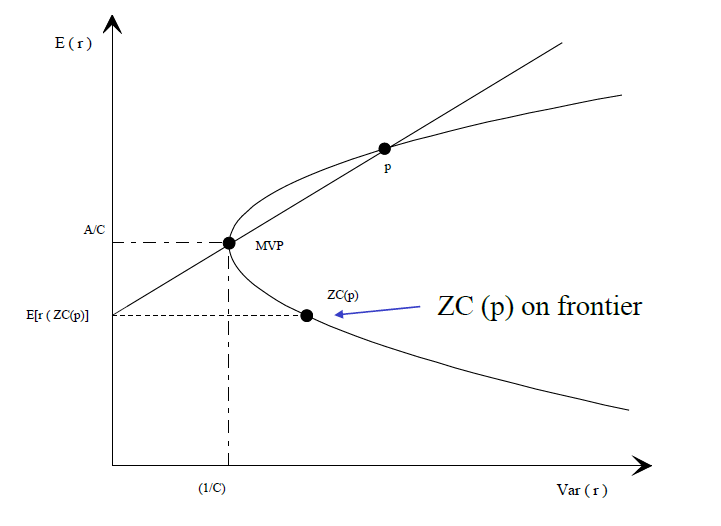
\includegraphics[scale=0.6]{4C__Users_tkpme_Dropbox_BookPCRA_Springer_Produ___D_Portfolio_Theory_Plots_zeroBetaPort_graph.PNG}
\par\end{centering}
\caption{Relationship between portfolios $p$, $p_{gmv}$ and $zc(p)$ in mean
return versus variance coordinates.}

\label{fig: zero-covariancePortfolioGeometry}
\end{figure}

It can be shown that the straight line in the above figure is given
by

\begin{equation}
\mu_{r}=\mu_{zc(p)}\,+\,\dfrac{\mu_{p}\,-\,\mu_{gmv}}{\sigma_{p}^{2}\,-\,\sigma_{gmv}^{2}}\,\sigma_{r}^{2}\label{eq: zc(p) geometry}
\end{equation}

and that $\mu_{r}=\mu_{gmv}$ when $\sigma_{r}^{2}=\sigma_{gmv}^{2}$.

\section{Proof of the APT\label{sec: APTproof}}

The vector $\mathbf{a}=(a_{1},\,a_{2},\,\cdots\,,\,a_{n})^{\prime}$
of intercepts in \APTintercepts\  may be written in the least-squares
regression fit-plus-residuals form

\begin{equation}
\begin{alignedat}{1}\mathbf{a} & =\hat{\lambda}_{0}\mathbf{1}\,+\,\text{\ensuremath{\mathbf{B}}\ensuremath{\ensuremath{\hat{\boldsymbol{\lambda}}}}}\,+\,\ensuremath{\mathbf{u}}\end{alignedat}
\label{eq: LSregression-avec-on-Bmat}
\end{equation}

where $\hat{\lambda}_{0}$ and $\hat{\boldsymbol{\lambda}}=(\hat{\lambda}_{1},\,\hat{\lambda}_{2},\,\cdots\,,\,\hat{\lambda}_{K})^{\prime}$
are the least-squares regression coefficients, and $\ensuremath{\mathbf{u}}=(u_{1},\,u_{2},\,\cdots\,,\,u_{n})^{\prime}$
is the vector of regression residuals. For details on the above LS
regression decomposition see \LeastSquaresSection, where it is shown
that the regression residuals vector $\ensuremath{\mathbf{u}}$ is
orthogonal to the vector $\mathbf{1}$ as well as to the columns of
$\mathbf{B}$. Thus $\mathbf{u}^{\prime}\mathbf{1}=\sum_{i\,=\,1}^{n}u_{i}=0$,
and $\mathbf{u}^{\prime}\mathbf{B}=\mathbf{0}^{\prime}$ where the
right hand side is a vector of $K$ zeros. It follows of course that
$\mathbf{u}$ is orthogonal to the fit $\mathbf{a}=\hat{\lambda}_{0}\mathbf{1}+\text{\ensuremath{\mathbf{B}}\ensuremath{\ensuremath{\hat{\boldsymbol{\lambda}}}}}$.

Consider the zero investment portfolio weights vector

\begin{equation}
\mathbf{w=}\frac{\ensuremath{\mathbf{u}}}{\sqrt{n}\mathrm{\left\Vert \ensuremath{\mathbf{u}}\right\Vert }}
\end{equation}

where $\left\Vert \ensuremath{\mathbf{u}}\right\Vert =\sqrt{\sum_{i\,=\,1}^{n}u_{i}^{2}}$.
Then using \APTreturnsModel\  along with the fact that $\mathbf{u}^{\prime}\mathbf{B}=\mathbf{0}^{\prime}$,
the arbitrage portfolio $p$ has return

\begin{align}
r_{p} & =\mathbf{w}^{\prime}\mathbf{r}\nonumber \\
 & =\dfrac{1}{\sqrt{n}\left\Vert \ensuremath{\mathbf{u}}\right\Vert }(\mathbf{u}^{\prime}\mathbf{a}\,+\,\mathbf{u}^{\prime}\bueps)\label{eq: arbPortfolioReturn}
\end{align}

and since $\mathrm{E}(\bueps)=0$, the arbitrage portfolio has mean

\begin{align}
\mu_{p} & =\dfrac{\mathbf{u}^{\prime}\mathbf{a}}{\sqrt{n}\left\Vert \ensuremath{\mathbf{u}}\right\Vert }\nonumber \\
 & =\dfrac{\mathbf{u}^{\prime}\ensuremath{\mathbf{u}}}{\sqrt{n}\left\Vert \ensuremath{\mathbf{u}}\right\Vert }\nonumber \\
 & =\dfrac{1}{\sqrt{n}}\left\Vert \ensuremath{\mathbf{u}}\right\Vert \label{eq: arbPorMean}
\end{align}

where the second line is due to substituting \eqref{eq: LSregression-avec-on-Bmat}
for $\mathbf{a}$ and using the orthogonality of $\mathbf{u}$ to
$\mathbf{1}$ and $\mathbf{B}$, and the last line is because $\mathbf{u}^{\prime}\ensuremath{\mathbf{u}}=\left\Vert \ensuremath{\mathbf{u}}\right\Vert ^{2}$.

The variance of the arbitrage portfolio $r_{p}$ is

\begin{align}
\mathrm{E}(r_{p}-\mu_{p})^{2} & =\mathrm{E}\left(\dfrac{\mathbf{u}^{\prime}\bueps}{\sqrt{n}\left\Vert \ensuremath{\mathbf{u}}\right\Vert }\right)^{2}\nonumber \\
 & =\dfrac{\mathbf{u}^{\prime}\mathbf{C}\mathbf{u}}{n\left\Vert \ensuremath{\mathbf{u}}\right\Vert ^{2}}\label{eq: arbPortRisk}
\end{align}

where $\mathbf{C}$ is the covariance matrix of the errors $\bueps=(\epsilon_{1},\,\epsilon_{2},\,\cdots,\,\epsilon_{n})^{\prime}$.
We say that the arbitrage portfolio is \emph{asymptotically risk diversifiable
}(ARD) if

\begin{equation}
\underset{n\rightarrow\infty}{\lim}\dfrac{\mathbf{u}^{\prime}\mathbf{C}\mathbf{u}}{n\left\Vert \ensuremath{\mathbf{u}}\right\Vert ^{2}}=0.\label{eq: asympRiskDiversifiable}
\end{equation}

The simplest condition that results in ARD is where the $\epsilon_{i}$
are uncorrelated and have bounded variances $\sigma_{i}^{2}<B$, for
in that case $\mathbf{u}^{\prime}\mathbf{C}\mathbf{u}=\sum_{i\,=\,1}^{n}u_{i}^{2}\sigma_{i}^{2}<B\sum_{i\,=\,1}^{n}u_{i}^{2}$
and the above ratio is bounded by $B/n$, which goes to 0 as $n\rightarrow\infty$.

Suppose the portfolio is ARD and that 

\begin{align*}
\mu_{p,\,\infty} & =\underset{n\rightarrow\infty}{\lim}\dfrac{1}{\sqrt{n}}\left\Vert \ensuremath{\mathbf{u}}\right\Vert \\
 & =\underset{n\rightarrow\infty}{\lim}\left(\dfrac{1}{n}\sum_{i\,=\,1}^{n}u_{i}^{2}\right)\\
 & >0.
\end{align*}

In that case, the arbitrage portfolio has an asymptotic sure profit
with no risk. But in a market that is arbitrage free this is not possible,
and it must be that the APT condition
\[
lim_{n\rightarrow\infty}\left(\dfrac{1}{n}\sum_{i\,=\,1}^{n}u_{i}^{2}\right)=0
\]
is satisfied.

\medskip{}


\section{Robust Estimation Details\label{sec: robEstDetails}}

\subsection{mOpt Psi Function Formula \label{subsec: boundedRhoPsiFormula}}

The mOpt psi function formula is

\begin{equation}
\psi_{mOpt}(x)=\begin{cases}
x & |x|\leqslant1\\
\dfrac{\phi(1)}{\phi(1)\,-\,a}\left(x\,-\,\mathrm{SGN}(x)\dfrac{a}{\phi(x)}\right)\mathrm{\mathit{U}}(c\,-\,|x|) & |x|>1
\end{cases}
\end{equation}

where $\phi(x)$ is the standard normal density function, $\mathrm{\mathit{U}}(x)$
is the unit step function whose value is 1 for $x\geqslant0$ and
is 0 for $x<0$, and the constants $a$ and $c$ depend on the desired
normal distribution efficiency. Note that $\psi_{mOpt}(x)=0$ for
$x$ outside the interval $(-c,\,c)$. A 95\% normal distribution
efficiency is obtained with $a=0.0132$ and $c=3.004$. The rho function
$\rho_{mOpt}(x)$ is obtained by an integration of $\psi_{mOpt}(x)$,
and because the latter is zero outside the interval $(-c,\,c)$, the
rho function is bounded with a constant value outside that interval.
Details of the integral of the mOpt psi function, and computing values
of $a$ and $c$ from specified normal distribution efficiencies are
provided in \citet{KonisMartin2021}.

\end{appendices}

\pagebreak{}

\begin{flushleft}
\printbibliography
\par\end{flushleft}

\newpage
\end{document}
